
% xetex expected
\documentclass[xetex,professionalfont]{beamer}

% we want math
\usepackage{amsmath}

% fixes and extensions to amsmath
\usepackage{mathtools}

% additional math symbols
\usepackage{amssymb}

% good-looking fractions in text via \sfrac
\usepackage{xfrac}

% fix spaces after custom commands (see below for examples)
\usepackage{xspace}

% minted allows for fancy syntax highlighting (requires python with pygments)
% usage:
%   \begin{minted}{python}
%   codeb
%   \end{minted}
\usepackage{minted}

% better looking tables
% usage:
%   begin with a \toprule, write a single row of column headings,
%   then add \midrule and after the columns of data we finish with \bottomrule
% example:
%   \begin{tabular}{llr} \toprule
%   Animal & Description & Price \midrule
%   cat & foo & 10 \\
%   dog & bar & 20 \\ \bottomrule
%   \end{tabular}
% note that good tables generally neither have vertical rules nor double rules
\usepackage{booktabs}

% support for figures
% example:
%   \begin{figure}
%   \centering
%   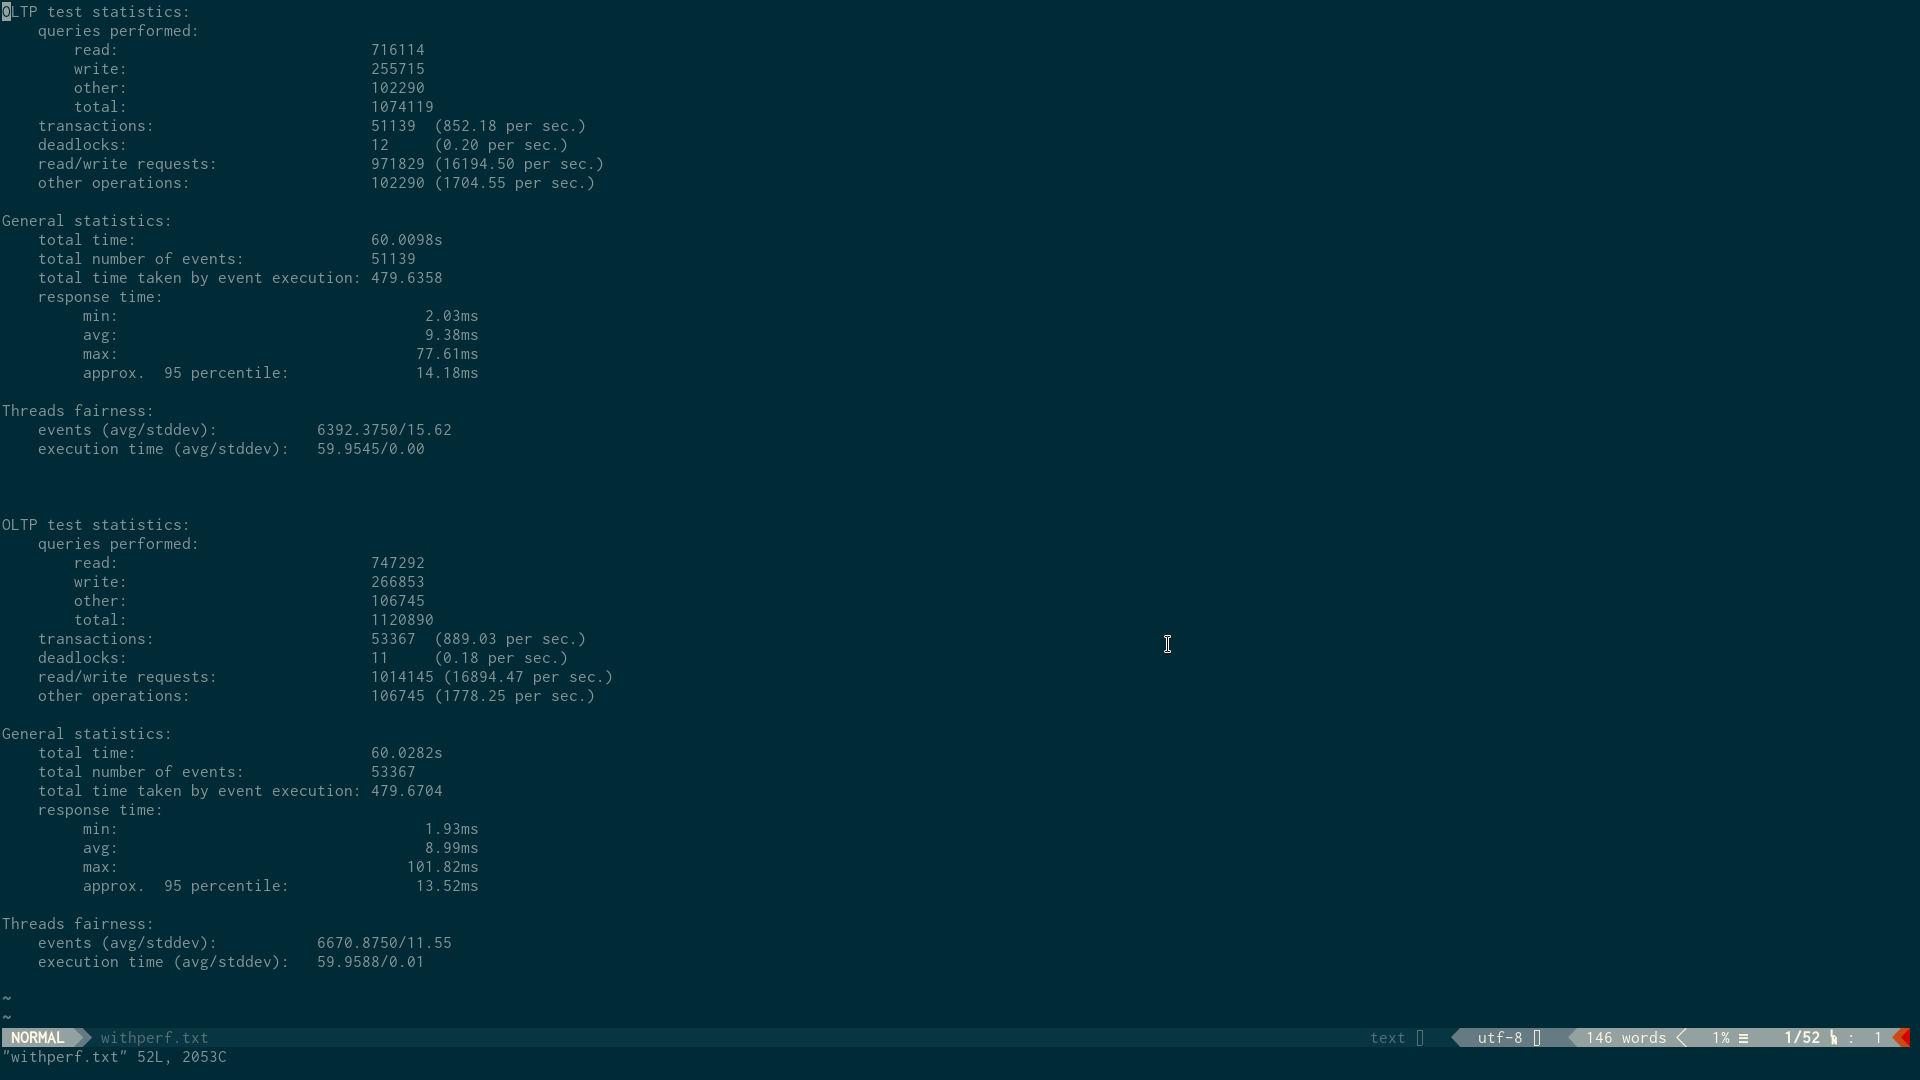
\includegraphics[width=0.5\textwidth]{image}}
%   \caption{my image}
%   \label{fig:image}
%   \end{figure}
% \usepackage{graphicx} % already loaded by beamer

% system font support (requires xetex or luatex)
\usepackage{fontspec}
\setsansfont{Roboto} % part of ttf-roboto on Arch
\setmonofont[Scale=0.7]{Cousine} % part of ttf-chromeos fonts on Arch

% subfigures
% example:
%   \begin{figure}
%   \centering
%   \subfloat[Cat\label{fig:cat}]{\includegraphics[width=0.4\textwidth]{cat}}\quad
%   \subfloat[Dog\label{fig:dog}]{\includegraphics[width=0.4\textwidth]{dog}}
%   \caption{Animals}
%   \label{fig:animals}
%   \end{figure}
\usepackage[caption=false]{subfig}
\captionsetup{belowskip=0pt,aboveskip=0pt}

% improve microtypography
\usepackage{microtype}

% multi-language quotes for babel
\usepackage{csquotes}

% easy way to include copyright information
\usepackage{copyrightbox}

% language support (english,ngerman)
\usepackage[english]{babel}

% better bibliographies
\usepackage[backend=biber,style=numeric]{biblatex}

% -----------------------------------------------------------------------------

% % specify PDF metadata
\hypersetup{pdftitle={CVL Beamer Template},pdfsubject={},pdfauthor={Christopher Pramerdorfer}}

% copyright font style
\makeatletter\renewcommand{\CRB@setcopyrightfont}{\tiny\color{lightgray}}

% make emph bold
\DeclareTextFontCommand{\emph}{\bfseries}

% use proper fonts for math
\usefonttheme[onlymath]{serif}

% use tuwcvl beamer theme
\usetheme{tuwcvl}

% -----------------------------------------------------------------------------

% common english abbreviations
\newcommand{\ie}{\mbox{i.e.}\xspace} % i.e.
\newcommand{\eg}{\mbox{e.g.}\xspace} % e.g.

% math - argmin and argmax
\DeclareMathOperator*{\argmin}{arg\,min}
\DeclareMathOperator*{\argmax}{arg\,max}

% shortcuts for number ranges
\newcommand{\NN}{\mathbb{N}}
\newcommand{\ZZ}{\mathbb{Z}}
\newcommand{\QQ}{\mathbb{Q}}
\newcommand{\RR}{\mathbb{R}}

% bold vectors
\renewcommand{\vec}[1]{\ensuremath{\mathbf{#1}}}

% vector shortcuts
\newcommand{\va}{\vec{a}}
\newcommand{\vb}{\vec{b}}
\newcommand{\vc}{\vec{c}}
\newcommand{\ve}{\vec{e}}
\newcommand{\vr}{\vec{r}}
\newcommand{\vs}{\vec{s}}
\newcommand{\vt}{\vec{t}}
\newcommand{\vu}{\vec{u}}
\newcommand{\vv}{\vec{v}}
\newcommand{\vw}{\vec{w}}
\newcommand{\vx}{\vec{x}}
\newcommand{\vy}{\vec{y}}
\newcommand{\vz}{\vec{z}}

% -----------------------------------------------------------------------------

\title{CVL Beamer Template}
\subtitle{My Subtitle}
\author{Christopher Pramerdorfer}
\institute{Computer Vision Lab, Vienna University of Technology}

\begin{document}

% -----------------------------------------------------------------------------

\begin{frame}
\maketitle
\end{frame}

% -----------------------------------------------------------------------------

\begin{frame}
\frametitle{First Slide}

First example slide.

Some interesting content.

\begin{itemize}
    \item First item
    \item Second item
\end{itemize}

Some math, $v=\sum_k x_k^2$.

% -----------------------------------------------------------------------------

\end{frame}

\begin{frame}[fragile]
\frametitle{Second Slide}
\framesubtitle{Some Subtitle}

Some \emph{interesting} code:

\begin{minted}{python}
def foo(x):
    return np.array(x, dtype=float)
\end{minted}

\end{frame}

% -----------------------------------------------------------------------------

\begin{frame}
\frametitle{Third Slide}

Have a look at Figure \ref{fig:tuwcvl}.

\begin{figure}
\centering
\copyrightbox[b]{
\includegraphics{tuwcvl.png}}{\centering Source logos are \copyright\ TU Wien \& CVL} 
\caption{Collection of logos.}
\label{fig:tuwcvl}
\end{figure}

Remaining text.

\end{frame}

% -----------------------------------------------------------------------------

\begin{frame}
\frametitle{Fourth Slide}

\begin{columns}
\column{0.5\textwidth} % beamer slides are 128mm by 96mm

Some text

Some more text

\column{0.4\textwidth}

\begin{center}

\includegraphics[width=3cm]{tuwcvl.png}\\
\vspace{1cm}

\includegraphics[width=3cm]{tuwcvl.png}\\
\vspace{1cm}

\includegraphics[width=3cm]{tuwcvl.png}
\end{center}

\end{columns}

\end{frame}

\end{document}